% Nome do capítulo
\chapter{Digital Image Processing}
% Label para referenciar
\label{cap3_seg_imagens}

% Diminuir espaçamento entre título e texto
%\vspace{-1.9cm}

% Texto do capítulo
Segmentation consists of subdividing an image into its constituent regions or objects \cite[Ch. 10]{gonzalez2002digital}.
It is also an important step in trying to explain an image through algorithms \cite{Zhang08imagesegmentation}. 
This chapter presents the main concepts related to image segmentation,
The division of this chapter is based on \cite{gonzalez2018digital} and \cite{pedrini2008analise} classification proposals.

The organization of the chapter is divided as follows: Section \ref{cap3_detect_bordas_segment} contains concepts of image segmentation;
Section \ref{cap3_morf_matematica} contains mathematical morphology methods for image processing and noise filtering;
and Section \ref{cap3_metricas_avaliacao} shows segmentation evaluation techniques.
%--------------------------------

%--------------------------------
%DETECÇÃO DE BORDAS E REGIÕES
\section{Image Segmentation}
\label{cap3_detect_bordas_segment}

%review pag. 151 PEDRINI
Conventional segmentation approaches are generally based on two basic image characteristics: discontinuity, a property that enables partitioning according to abrupt tonal changes, and similarity, which allows grouping of points with similar values.
When image analysis uses information to identify groups, such as labels or ground truths, the analysis process is said to be supervised; when labels are not used, the process is called unsupervised \cite{gonzalez2002digital}. %\cite{pedrini2008analise} .

%DETECÇÃO DE DESCONTINUIDADES
\subsection{Discontinuity Detection}
\label{cap3_descontinuidades}

Discontinuity detection seeks to identify points, line segments, junctions, and edges, which are considered basic structures in digital images.
Discontinuity detection is commonly done by applying masks in the figure, such as low pass filters, high pass filters, and convolutions  \cite{gonzalez2002digital}. %\cite{pedrini2008analise}
%In this section, the focus will be given only to edge detection, object of study of this work.

A boundary is a set of connected pixels that border two regions \cite{gonzalez2002digital}.
Since borders constitute abrupt changes in the color threshold between regions, it can be described them using derivatives.
The gradient, denoted by $\nabla f$ or \textbf{grad} $f$, gives the biggest growing direction of a function $f$ \cite{stewart2003calculus}. 
The gradient vector $\nabla f(x_0 , y_0 )$ is always perpendicular to the tangent direction of the border \cite{stewart2003calculus}. % \cite{pedrini2008analise}.

For a two-variable function $x$ and $y$, with standard unit vectors $i$ and $j$ in the directions of $x$ and $y$, $\nabla f(x,y)$ is defined by Equation \ref{eq:cap3_gradiente}:

% \cite{stewart2003calculus}
\begin{equation}
 \nabla f(x,y)= \langle G_x, G_y \rangle = \langle f_x (x,y), f_y (x,y) \rangle = \frac{\partial f}{\partial x}i + \frac{\partial f}{\partial y}j
 \label{eq:cap3_gradiente}
\end{equation}

% \cite{pedrini2008analise}
The magnitude of the gradient vector corresponds to the rate of greatest variation of the gradient $G$, in directions $x$ and $y$, denoted by $mag(\nabla f)$, and defined by Equation \ref{eq:cap3_mag_gradiente}: 

\begin{equation}
 mag(\nabla f)= \sqrt{\left(G_x^2 + G_y^2 \right)} = \sqrt{ \left(\frac{\partial f}{\partial x} \right)^2 + \left(\frac{\partial f}{\partial y} \right)^2}
 \label{eq:cap3_mag_gradiente}
\end{equation}

% \cite{pedrini2008analise}
The direction of the gradient, measured relative to the $x$ axis, is given by Equation \ref{eq:cap3_theta_gradiente}:

\begin{equation}
 \theta (x,y) = arctan \left(\frac{G_y}{G_x} \right)
 \label{eq:cap3_theta_gradiente}
\end{equation}

Using the equations previously described in Section it is possible to detect boundaries.
Vertical edges can be detected by the horizontal difference between points, that is, by the derivatives with respect to the axis $x$; while horizontal edges can be detected by derivatives relative to the axis $y$ \cite{pedrini2008analise}.

\subsubsection{Boundary Detection}
\label{cap3_boundary_detection}

Edge corresponds to an abrupt change in an image aspect, like color or brightness.
Boundary is a higher feature, related to the limits between objects or regions in an image.
The relationship between them emerge from the common use of edge detection techniques, grouping fragments of edges into contours, to produce boundary detection \cite{MARTIN:1273918}.

Traditional approaches of boundary detection uses filter masks, gradients or evaluates image brightness discontinuities.
These methods, however, are inadequate for natural boundaries, that contains texture inside a object (does not produce an boundary) and 
a subtle brightness between two or more objects (producing a boundary) \cite{MARTIN:1273918} \cite[Ch. 10]{gonzalez2002digital}.

%In recent years, some methods of edge and boundary detection have emerged, using convolutional neural networks, as will be detailed in Section \ref{cap4_trab_rel}.

%SUB - SEGMENTAÇÃO UTILIZANDO REDES NEURAIS
\subsubsection{Region Segmentation}
\label{cap3_redes_neurais_seg}

Region segmentation seeks to identify sets of pixels (regions) directly in images.
Traditional methods use region growing and watersheds.
Other methodologies allow for segmentation of regions using superpixels, $k$-means clusters and graph cuts \cite{pedrini2008analise}.

Approaches to image segmentation using convolutional neural networks have emerged in the past few years.
Neural networks allow features to be learned by special algorithms, that does not require explicit programming, unlike previous methods, which required imperative programming \cite{Segnet:2017:7803544}.

Automatic feature learning enables the identification and matching of patterns, generating results with techniques not initially foreseen.
On the downside, the networks are unable to explain the patterns identified, despite the existence of research to solve this problem \cite{Segnet:2017:7803544} \cite{Yosinski:2015}.
%--------------------------------

%--------------------------------
%MORFOLOGIA MATEMÁTICA
\section{Mathematical Morphology}
\label{cap3_morf_matematica}

Mathematical morphology is a technique for analysis and processing of geometric structures based on set and lattice theories.
It is often used for feature analysis and construction of useful operators for object description.
Originally developed for binary image analysis, the techniques were subsequently extended to grayscale images \cite{Serra:2000} \cite{pedrini2008analise}.

Mathematical morphology contains a series of morphological operators, which can be used directly or in combination, for more complex activities.
These operations are performed on images with the aid of sets of pixels in different shapes and sizes, called structuring elements.
Its purpose is to interact and verify how the shape of the element fits into an image by hitting or losing pixels (Hit-or-Miss transform) \cite{Dougherty:1992} \cite{Serra:2000}.

Elemental morphological operations correspond to expansion and erosion operations, from which other operations derive.
These operations can be formally defined by Minkowski's algebra adopted in set theory.
The dilation operator between a set $A$ and a structural element $E$ corresponds to the Minkowski addition operation, while the erosion operator corresponds to the Minkowski subtraction operation. \cite{pedrini2008analise}.

Minkowski addition is defined according to Equation \ref{eq:cap3_morf_dilat}, corresponding to the set of all $E$ translations in $A$ where there is at least one non-null element in common with the $A$ set \cite{pedrini2008analise}.

\begin{equation}
 \textit{dilation}(A,E) = A \oplus E = \bigcup_{e \in E} (A + e)
 \label{eq:cap3_morf_dilat}
\end{equation}

Minkowski subtraction is defined according to Equation \ref{eq:cap3_morf_eros}, corresponding to the set of all $E$ elements translated by $p$ that are contained in $A$ \cite{pedrini2008analise}.

\begin{equation}
 \textit{erosion}(A,E) = A \ominus E = \bigcap_{e \in E} (A - e)
 \label{eq:cap3_morf_eros}
\end{equation}

Simply put, dilation increases the size of light regions of the image and reduces dark regions.
In turn, erosion performs the reverse procedure: it reduces the size of bright regions of the image and widens dark regions \cite[Ch. 9]{HIPR:1996}.
Figure \ref{fig:cap3_morph_dilat_eros} displays the result of dilation and erosion operations on an image using a rectangular structuring element of $7 \times 7$.

\begin{figure}
  \centering
  \caption{Original image (a), after morphological dilation (b) and erosion (c).}
  \subfloat[\label{fig:cap3_morph_dilat_eros_1}]{
\includegraphics[width=0.22\textwidth]{imagens/ilustracoes/cap3_morphology_original.png}}
  \hfill
  \subfloat[\label{fig:cap3_morph_dilat_eros_2}]{
\includegraphics[width=0.22\textwidth]{imagens/ilustracoes/cap3_morphology_dilatacao.png}}
  \hfill
  \subfloat[\label{fig:cap3_morph_dilat_eros_3}]{
\includegraphics[width=0.22\textwidth]{imagens/ilustracoes/cap3_morphology_erosao.png}}
  \sourceOwn
  \label{fig:cap3_morph_dilat_eros}
\end{figure}

In addition to the previously mentioned operations, the morphological opening and closing operations stand out in the literature.
The opening operation is obtained by erosion of an image, followed by dilation; while closure is achieved by dilation followed by erosion.
Opening is intended to remove small objects or noise, while closing seeks to close small holes in the background of the image \cite{pedrini2008analise}.
Figure \ref{fig:cap3_morph_close_open} shows both operations.

\begin{figure}
  \centering
  \caption{Morphological opening (a) and closing (b) operations.}
  \subfloat[\label{fig:cap3_morph_close_open_1}]{
\includegraphics[width=0.45\textwidth]{imagens/ilustracoes/cap3_morphology_abertura.png}}
  \hfill
  \subfloat[\label{fig:cap3_morph_close_open_2}]{
\includegraphics[width=0.45\textwidth]{imagens/ilustracoes/cap3_morphology_fechamento.png}}
  \sourceOwn
  \label{fig:cap3_morph_close_open}
\end{figure}

Also noteworthy is the morphological thinning operation.
This operation aims to reduce components connected to elements of a single pixel wide, maintaining the shape of the original image \cite{Abhishek:2017}.
Figure \ref{fig:cap3_morph_thin} shows the result of the morphological thinning operation.

\begin{figure}
  \centering
  \caption{Morphological thinning operation.}
  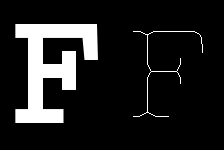
\includegraphics[width=0.45\textwidth]{imagens/ilustracoes/cap3_morphology_thin.png}
  \sourceOwn
  \label{fig:cap3_morph_thin}
\end{figure}
%--------------------------------

%--------------------------------
%MÉTRICAS DE AVALIAÇÃO
\section{Evaluation Metrics}
\label{cap3_metricas_avaliacao}

In order to evaluate segmentation effectiveness, subjective methods have traditionally been used, such as human visual perception, which is responsible for comparing the quality of computationally produced segmentation with a manually segmented image \cite{Zhang08imagesegmentation}. Due to the subjectivity of the method, different techniques were developed to compare quality and efficiency, as will be shown in this chapter. 

Firstly, in decision problems the classifiers can be positive or negative \cite{DavisGoadrich:2006}. 
The decision made by a classifier can be represented by a structure known as a confusion matrix or contingency table.
According to \cite{DavisGoadrich:2006}, it can identify 4 possible data types:

\vspace{-0.2cm}
\begin{itemize}
 \item \textit{True Positives (TP)}: values that were correctly classified as positive;
 \item \textit{False Negatives (FN)}: values that were incorrectly classified as negative;
 \item \textit{False Positives (FP)}: values that were incorrectly classified as positive;
 \item \textit{True Negatives (TN)}: values that were correctly classified as negative.
\end{itemize}

From the classification of results, it is possible to generate quality evaluation metrics.
The simplest metrics correspond to false positive and false negative rates \cite{Fawcett:2006}.
\ac{FPR} corresponds to the amount of incorrectly classified positive values $FP$ over the number of negative pixels $N$ and 
\ac{FNR} corresponds to the amount of incorrectly classified negative values $FN$ over the number of positive pixels $P$ \cite{Fawcett:2006}.

\begin{equation}
  \centering
  \label{equ:cap3_false_rate}
  \begin{aligned}
    FPR = \frac{FP}{N} \qquad\qquad
    FNR = \frac{FN}{P} 
  \end{aligned}
\end{equation}

Also, \ac{TPR} corresponds to the amount of correctly rated positive values $TP$ over the number of positive pixels $P$ and  
\ac{TNR} corresponds to the amount of correctly rated negative values $TN$ over the number of negative pixels $N$. 
The error rate is the number of incorrectly classified positive and negative over the sum of pixels \cite{Guo:2012}.

\begin{equation}
  \centering
  \label{equ:cap3_true_rate}
  \begin{aligned}
    TPR = \frac{TP}{P} \qquad\qquad
    TNR = \frac{TN}{N} 
  \end{aligned}
\end{equation}

\begin{equation}
  Error~rate = \frac{FP+FN}{P + N}
  \label{equ:cap3_error_rate}
\end{equation}

The accuracy, according \cite{Smith:1997:SEG:281875} and \cite{Fawcett:2006} is defined as ``the difference between the actual value and the average of the underlying process that generates the data''. 
Corresponds to true positive rate $TP$, added to the true negative rate $TN$, over the sum of positive $P$ and negative $N$ pixels, as Equation \ref{equ:cap3_acuracia}.

\begin{equation}
  accuracy = \frac{TP+TN}{P+N}
  \label{equ:cap3_acuracia}
\end{equation}

Precision and recall are binary classification metrics, where precision measures the proportion of model events that are true; while recall measures the proportion of events that occur in the domain that are captured by the models \cite{TorgoRibeiro:2009} \cite{Fawcett:2006}. 
%Both measures are formally described in Equation \ref{equ:cap3_precision_recall}. %\ref{equ:cap3_precision} and \ref{equ:cap3_recall}.

\begin{equation}
  precision = \frac{TP}{TP+FP}
  %\label{equ:cap3_precision}
\end{equation}

\begin{equation}
  recall = \frac{TP}{TP+FN}
  \label{equ:cap3_recall}
\end{equation}

For a simple confusion matrix, F-measure, also called F-score, is a harmonic mean of precision and recall, defined as Equation \ref {equ:cap3_f_measure} \cite{Fawcett:2006}.

\begin{equation}
  \text{\textit{F-measure}} = \frac{2 \cdot precision \cdot recall}{precision + recall}
  \label{equ:cap3_f_measure}
\end{equation}

%--------------------------------
%MÉTRICAS PARA CLASSIFICAÇÃO DE PIXELS
\subsection{Pixel Classification Metrics}
\label{cap3_metricas_pixels}

For classification problems, F-measure is a harmonic mean that imposes a better balance between accuracy and recall, and is therefore best suited for unbalanced data \cite{DavisGoadrich:2006}. 
Given a binary $m$-dimensional vector and associated accuracy and recall classes, the F-measure is given by Equation \ref{equ:cap3_fmeasure} \cite{DavisGoadrich:2006}.

\begin{equation}
 F=\frac{ 2 \sum\limits_{i=1}^m {precision_i \cdot recall_i}}{ \sum\limits_{i=1}^m {precision_i} + \sum\limits_{i=1}^m {recall_i}}  \in [0,1] 
 \label{equ:cap3_fmeasure}
\end{equation}

\ac{ROC} is a graphical representation that shows the performance of a binary classifier.
The curve shows the variation of positive samples correctly classified relative to the number of incorrectly classified ones.
In this chart, the Cartesian axis $y$ corresponds to the rate of true positives, while the $x$ axis is related to false positive rate \cite{Fawcett:2006}.

Related to \ac{ROC} curve, it is possible to define \textit{sensitivity} as the same concept of recall and \textit{specificity} as the number of true negatives over the sum of false positive and true negative values \cite{Fawcett:2006}.

\begin{equation}
  specificity  = \frac{TN}{FP + TN}
  \label{equ:cap3_specificity}
\end{equation}

\ac{PR} curves are parametric curves that assess the balance between accuracy and noise for different threshold values of a detector \cite{MARTIN:1273918}.
\ac{AUC} is the area under \ac{ROC} curve (\ac{AUC}-ROC) or \ac{PR} curve (\ac{AUC}-PR), and high values indicates both high recall and high precision values \cite{DavisGoadrich:2006} \cite{Sofaer:2019}. 

A metric called \textit{Pixel-error} rounds values between 0 to 1 interval and measures the number of misclassified pixels with over the total number of pixels. 
This measure can be considered the easiest way to compute pixel-wise boundary prediction errors \cite{Unet:2015} \cite{ISBI:2012} \cite{ArgandaCarreras:2015}.

\begin{equation}
  \text{\textit{Pixel-error}} = \nint*{\frac{FN + FP}{N + P}}
  \label{equ:cap3_pixel_error}
\end{equation}

%--------------------------------
%MÉTRICAS PARA CLASSIFICAÇÃO DE SEGMENTAÇÕES
\subsection{Segmentation Classification Metrics}
\label{cap3_metricas_segmentacao}

Segmentation metrics measure efficiency based on contours, pair of pixels or regions.
Contours-based methods evaluates the boundaries between foreground objects and the background; 
pair-of-pixels methods evaluate whether a pair of pixels belong to the same or different regions;
and region methods analyze sets of pixels grouped into regions \cite{Pont-Tuset2016a}.

For contour evaluation, techniques based on mathematical morphology are frequently used.
This is done by ground truth pixel dilations, counting the edge objects that cross the resulting mask, and then calculating the morphological F-measure for edges \cite{Pont-Tuset2016a}.

Frequently, two metrics, \ac{ODS} and \ac{OIS}, are used in contour evaluation.
\ac{ODS} is the metric used when a fixed threshold (\acused{TH}\ac{TH}) is adjusted to provide optimal performance for all images on the training set.
\ac{OIS} is the metric used when the threshold is defined per image, by an oracle \cite{amfm_pami2011}.

% For pair of pixels method, partitions are used to evaluate the results.
% Considering $\mathcal{S}$ and $\mathcal{S'}$ two segments, it can be divided in a set of $\mathcal{P}$ pixel pairs into subsets, formed by pixels combination that are in the same or different regions of each of the segments $S$ and $S'$.
% The Rand Index  $(IR)$ is frequently used, where $\mathcal{P}_{11}$ represents pixels in the same region in $S$ and $S'$, and $\mathcal{P}_{00}$ represents pixels in different regions in $S$ and $S'$ \cite{Pont-Tuset2016a} \cite{Rand:1971} \cite{Meila:2005}.

For pair of pixels method, partitions are used to evaluate the results.
Considering $\mathcal{S}$ and $\mathcal{S'}$ two segments, it can be divided in a set of $\mathcal{P}$ pixel pairs into 4 subsets, formed by pixels combination that are in the same or different regions of each of the segments $S$ and $S'$ \cite{Meila:2005} \cite{Pont-Tuset2016a}.

The Rand Index \cite{Rand:1971} $(IR)$, defined by Equation \ref{equ:cap3_rand_method}, is used for pixel classification, where $\mathcal{P}_{11}$ represents pixels in the same region in $S$ and $S'$, and $\mathcal{P}_{00}$ represents pixels in different regions in $S$ and $S'$ \cite{Pont-Tuset2016a}.
The Rand index still has a probabilistic version known as \textit{Probabilistic Rand Index} (PRI) \cite{Milena:2019}.

\begin{equation}
 IR\mathcal{(S,S')} = \frac{|\mathcal{P}_{00}| + |\mathcal{P}_{11}|}{|\mathcal{P}|}
 \label{equ:cap3_rand_method}
\end{equation}

% For the classification of regions, highlights \ac{SC} and \ac{VoI} methods.
% Segmentation Covering (\ac{SC}) is a generalization of the Jaccard Index, that measures the overlap between two regions $\mathcal{R}$ and $\mathcal{R'}$.
% Variation of Information measures the distance between two clusters $\mathcal{S}$ and $\mathcal{S'}$, and evaluate the distance between them as the amount of information gained or lost when switching from one cluster to another \cite{Milena:2019} \cite{Pont-Tuset2016a} \cite{Meila:2003} \cite{amfm_pami2011}.

For the classification of regions, highlights, among several existing techniques, \ac{SC} \cite{amfm_pami2011} and \ac{VoI} \cite{Meila:2003} methods.
In both, it must be considered segmentations $S$ e $S'$. 
These metrics are intended to match each region of the $S$ with each region of the $S'$.

Variation of Information (\ac{VoI}) measures the distance between two clusters $\mathcal{S}$ and $\mathcal{S'}$.
The distance between them is the amount of information gained or lost when switching from one cluster to another \cite{Milena:2019} \cite{Meila:2005}
Considering that one cluster correspond to segmentation $\mathcal{S}$ and the other as ground truth $\mathcal{S'}$, the Variation of Information is given by Equation \ref{equ:cap3_voi}, where $\mathcal{H}$ is the entropy and $\mathcal{I}$ is the mutual information between the clusters.

\begin{equation}
 VoI\mathcal{(S, S') = H(S) + H(S')} − 2 \mathcal{I(S, S')}
 \label{equ:cap3_voi}
\end{equation}

Segmentation Covering (\ac{SC}), a generalization of the Jaccard Index, measures the overlap between two regions $\mathcal{R}$ and $\mathcal{R'}$ \cite{Milena:2019} \cite{Pont-Tuset2016a}.
In image evaluation, $\mathcal{R}$ is a region of the segmentation and $\mathcal{R'}$ is a ground truth region.
Equation \ref{equ:cap3_cobert_segm} shows the relationship between regions, where $n$ represents the number of pixels in an image.

\begin{equation}
 SC\mathcal{(S' \rightarrow S)} = \frac{1}{n} \sum\limits_{\mathcal{R} \in \mathcal{S}} {|\mathcal{R}|} \max\limits_{\mathcal{R'} \in \mathcal{S'}} \cdot \frac{|\mathcal{R} \cap \mathcal{R'}|}{|\mathcal{R} \cup \mathcal{R'}|}
 \label{equ:cap3_cobert_segm}
\end{equation}

Segmentation Covering for a set of $m$ ground truths is defined by average result of coverage of each $\mathcal{S}$ relative to each ground truth $\mathcal{G}_i$ separately \cite{Milena:2019}.

\begin{comment}

%--------------------------------
%MÉTRICAS PARA CLASSIFICAÇÃO DE SEGMENTAÇÕES
\subsection{\color{red}Segmentation Classification Metrics}
\label{cap3_metricas_segmentacao}

For contour evaluation, techniques based on mathematical morphology are frequently used.
This is done by ground truth pixel dilations, counting the edge objects that cross the resulting mask, and then calculating the morphological F-measure for edges \cite{Pont-Tuset2016a}.

For pair of pixels method, partitions are used to evaluate the results.
Considering $\mathcal{S}$ and $\mathcal{S'}$ two segments, it can be divided in a set of $\mathcal{P}$ pixel pairs into 4 subsets, formed by pixels combination that are in the same or different regions of each of the segments $S$ and $S'$ \cite{Meila:2005} \cite{Pont-Tuset2016a}.

The Rand Index \cite{Rand:1971} $(IR)$, defined by Equation \ref{equ:cap3_rand_method}, is used for pixel classification, where $\mathcal{P}_{11}$ represents pixels in the same region in $S$ and $S'$, and $\mathcal{P}_{00}$ represents pixels in different regions in $S$ and $S'$ \cite{Pont-Tuset2016a}.
The Rand index still has a probabilistic version known as \textit{Probabilistic Rand Index} (PRI).

\begin{equation}
 IR\mathcal{(S,S')} = \frac{|\mathcal{P}_{00}| + |\mathcal{P}_{11}|}{|\mathcal{P}|}
 \label{equ:cap3_rand_method}
\end{equation}

For the classification of regions, highlights, among several existing techniques, \ac{SC} \cite{amfm_pami2011} and \ac{VoI} \cite{Meila:2003} methods.
In both, it must be considered segmentations $S$ e $S'$. 
These metrics are intended to match each region of the $S$ with each region of the $S'$.

Variation of Information (\ac{VoI}) measures the distance between two clusters $\mathcal{S}$ and $\mathcal{S'}$.
The distance between them is the amount of information gained or lost when switching from one cluster to another \cite{Milena:2019} \cite{Meila:2005}
Considering that one cluster correspond to segmentation $\mathcal{S}$ and the other as ground truth $\mathcal{S'}$, the Variation of Information is given by Equation \ref{equ:cap3_voi}, where $\mathcal{H}$ is the entropy and $\mathcal{I}$ is the mutual information between the clusters.

\begin{equation}
 VoI\mathcal{(S, S') = H(S) + H(S')} − 2 \mathcal{I(S, S')}
 \label{equ:cap3_voi}
\end{equation}

Segmentation Covering (\ac{SC}), a generalization of the Jaccard Index, measures the overlap between two regions $\mathcal{R}$ and $\mathcal{R'}$ \cite{Milena:2019} \cite{Pont-Tuset2016a}.
In image evaluation, $\mathcal{R}$ is a region of the segmentation and $\mathcal{R'}$ is a ground truth region.
Equation \ref{equ:cap3_cobert_segm} shows the relationship between regions, where $n$ represents the number of pixels in an image.

\begin{equation}
 SC\mathcal{(S' \rightarrow S)} = \frac{1}{n} \sum\limits_{\mathcal{R} \in \mathcal{S}} {|\mathcal{R}|} \max\limits_{\mathcal{R'} \in \mathcal{S'}} \cdot \frac{|\mathcal{R} \cap \mathcal{R'}|}{|\mathcal{R} \cup \mathcal{R'}|}
 \label{equ:cap3_cobert_segm}
\end{equation}

Segmentation Covering for a set of $m$ ground truths is defined by average result of coverage of each $\mathcal{S}$ relative to each ground truth $\mathcal{G}_i$ separately \cite{Milena:2019}.
%--------------------------------
\end{comment}
